    \documentclass[twocolumn,
        nofootinbib, % unbreaks footnotes from being put in bib
        usenames, % allows access to some tikz colors
        aps,
        prd,
        dvipsnames % more colors: https://en.wikibooks.org/wiki/LaTeX/Colors
    ]{revtex4-1}% chktex 8
    \usepackage{
        amsmath,
        amssymb,
        fancyhdr, % page styling
        lastpage, % footer fanciness
        hyperref, % various links
        setspace, % line spacing
        amsthm, % newtheorem and proof environment
        mathtools, % \Aboxed for boxing inside aligns, among others
        float, % Allow [H] figure env alignment
        enumerate, % Allow custom enumerate numbering
        graphicx, % allow includegraphics with more filetypes
        wasysym, % \smiley!
        upgreek, % \upmu for \mum macro
        listings, % writing TrueType fonts and including code prettily
        tikz, % drawing things
        booktabs, % \bottomrule instead of hline apparently
        cancel % can cancel things out!
    }
    \usepackage[
        labelfont=bf, % caption names are labeled in bold
        font=scriptsize % smaller font for captions
    ]{caption}
    \usepackage[font=scriptsize]{subcaption} % subfigures

    \newcommand*{\scinot}[2]{#1\times10^{#2}}
    \newcommand*{\dotp}[2]{\left<#1\,\middle|\,#2\right>}
    \newcommand*{\rd}[2]{\frac{\mathrm{d}#1}{\mathrm{d}#2}}
    \newcommand*{\pd}[2]{\frac{\partial#1}{\partial#2}}
    \newcommand*{\rtd}[2]{\frac{\mathrm{d}^2#1}{\mathrm{d}#2^2}}
    \newcommand*{\ptd}[2]{\frac{\partial^2 #1}{\partial#2^2}}
    \newcommand*{\md}[2]{\frac{\mathrm{D}#1}{\mathrm{D}#2}}
    \newcommand*{\pvec}[1]{\vec{#1}^{\,\prime}}
    \newcommand*{\svec}[1]{\vec{#1}\;\!}
    \newcommand*{\ang}[0]{\;\text{\AA}}
    \newcommand*{\mum}[0]{\;\upmu \mathrm{m}}
    \newcommand*{\at}[1]{\left.#1\right|}

    \newtheorem{theorem}{Theorem}[section]

    \let\Re\undefined
    \let\Im\undefined
    \DeclareMathOperator{\Res}{Res}
    \DeclareMathOperator{\Re}{Re}
    \DeclareMathOperator{\Im}{Im}
    \DeclareMathOperator{\Log}{Log}
    \DeclareMathOperator{\Arg}{Arg}
    \DeclareMathOperator{\Tr}{Tr}
    \DeclareMathOperator{\E}{E}
    \DeclareMathOperator{\Var}{Var}
    \DeclareMathOperator*{\argmin}{argmin}
    \DeclareMathOperator*{\argmax}{argmax}
    \DeclareMathOperator{\sgn}{sgn}
    \DeclareMathOperator{\diag}{diag\;}

    \DeclarePairedDelimiter\bra{\langle}{\rvert}
    \DeclarePairedDelimiter\ket{\lvert}{\rangle}
    \DeclarePairedDelimiter\abs{\lvert}{\rvert}
    \DeclarePairedDelimiter\ev{\langle}{\rangle}
    \DeclarePairedDelimiter\p{\lparen}{\rparen}
    \DeclarePairedDelimiter\s{\lbrack}{\rbrack}
    \DeclarePairedDelimiter\z{\lbrace}{\rbrace}

    % \everymath{\displaystyle} % biggify limits of inline sums and integrals
    \tikzstyle{circ} % usage: \node[circ, placement] (label) {text};
        = [draw, circle, fill=white, node distance=3cm, minimum height=2em]
    \definecolor{commentgreen}{rgb}{0,0.6,0}
    \lstset{
        basicstyle=\ttfamily\footnotesize,
        frame=single,
        numbers=left,
        showstringspaces=false,
        keywordstyle=\color{blue},
        stringstyle=\color{purple},
        commentstyle=\color{commentgreen},
        morecomment=[l][\color{magenta}]{\#}
    }

\begin{document}

\def\Snospace~{\S{}} % hack to remove the space left after autorefs
\renewcommand*{\sectionautorefname}{\Snospace}
\renewcommand*{\appendixautorefname}{\Snospace}
\renewcommand*{\figureautorefname}{Fig.}
\renewcommand*{\equationautorefname}{Eq.}
\renewcommand*{\tableautorefname}{Tab.}

\begin{abstract}
    In white dwarf binaries tidal torques are expected to raise a train of
    internal gravity waves in the white dwarf interior. These
    outward-propagating waves can then grow to be nonlinear and break via
    hydrodynamical instabilities, transfering energy and angular momentum from
    the binary orbit to the white dwarf. We perform 2D numerical simulations of
    nonlinear wave breaking of outwards-propagating internal gravity waves in an
    incompressible, isothermal atmosphere with an exponentially decaying density
    stratification. We find that tidal synchronization, after an initial
    transient phase, proceeds inwards from the surface in thin layers. We argue
    the thickness of these layers is limited by the Kelvin-Helmholtz
    Instability. We provide simple analytical formulae for the location and
    thickness of tidal synchronization over time that are in good agreement with
    our simulations.
\end{abstract}

\title{Tidal Heating via Internal Gravity Waves in White Dwarf Binaries}
\author{Authors}
\date{\today}
\maketitle

\section{Introduction}

% Usual WD binaries introduction, from proposals

% IGW tidal dissipation has been thoroughly studied in many astrophysical
% binary systems (Barker Ogilvie, Goldreich Nicholson, Zahn?). Its effect in WDs
% (Fuller Lai) resembles early solar type stars but has not been studied
% numerically. While the linear IGW solution is an exact solution of the
% nonlinear system (Drazin) but is globally unstable (Drazin), the IVP must be
% studied numerically to determine how the linear solution breaks down and
% deposits energy/angular momentum.

% From numerical studies, IGWs are known to be anti-diffusive (Lecoanet mean
% flow papers, Lindzen) and sharpen mean flows (m = 0). Mean flows produce
% reflection, known both analytically (Booker & Bretherton) and numerically
% (Winters d'Asaro). IGW self-interaction via its wave-induced mean flow is
% known to play a crucial role in IGW wavebreaking (Sutherland x2).

% We study IGW breaking in the plane-parallel approximation in 2D. Known to
% describe both wave steepening (Kloyermeister 1991) and captures mean flow
% absorption (Booker & Bretherton). While the details of breaking are presently
% understood to be 3D (Winters & d'Asaro), we argue in (section) that our
% results should be qualitatively similar to 3D (both 2D and 3D exhibit KHI, and
% since we are able to resolve KHI, the spinup in 3D should be similar?).

In \autoref{s:equations}, we will cover the numerical setup. In \autoref{s:lin}, we
will discuss the agreement of our simulation in the low-amplitude limit with
analytical linear theory. In \autoref{s:nonlin} we will present a few reference
simulations illustrating critical layer absorption depositing horizontal angular
momentum into the fluid.

\section{Equations}\label{s:equations}

We consider an incompressible, isothermal fluid, representative of degenerate
matter in WD bulks, in 2D. We assume a barotropic equation of state as a first
approximation. As we are interested in the behavior of the wave far from the
center of the WD, we approximate the gravitational field as uniform. We model
the background density stratification as $\rho_0(x, z) = \rho_0(z) = \rho_0(z=0)
e^{-z/H}$ for some reference density $\rho_0(z=0) = \at{\rho_0(z)}_{z = 0}$.

The Euler equations for an incompressible, barotropic fluid in a uniform
gravitational field are
\begin{subequations}\label{se:fc_orig}
    \begin{align}
        \vec{\nabla} \cdot \vec{u} &= 0,\\
        \md{\rho}{t} &= 0 ,\label{eq:fc_density}\\
        \md{\vec{u}}{t} + \frac{\vec{\nabla}P}{\rho} + g\hat{z} &= 0.
    \end{align}
\end{subequations}
$\md{}{t} = \pd{}{t} + \p*{\vec{u} \cdot \vec{\nabla}}$ is the material
derivative. $\vec{u}, \rho, P$ are the fluid dynamical variables and $-g\hat{z}$
is constant gravitational acceleration. Note that at hydrostatic equilibrium
$\pd{}{t} = 0$ we have $\vec{\nabla}P_0 = -\rho_0 g\hat{z}$ and so $P_0 = \rho_0
gH$. A shear flow $u_x(x, z, t) = u_x(z)$ is permitted in hydrostatic
equilibrium, but we will initially consider no shear flow in equilibrium.

\section{Internal Gravity Waves: Linear Theory}

\subsection{Analytical Properties}

In the small perturbation limit, where flow velocities are small compared to the
characteristic space and time scales $\pd{}{t} \gg \vec{u} \cdot \vec{\nabla}$,
we linearize \autoref{se:fc_orig} by ignoring the advective components of the
material derivative, defining $\rho_1 \equiv \rho - \rho_0 \ll \rho_0 \ll
\rho_0$ and $P_1 \equiv P - P_0 \ll P_0$ deviations from equilibrium and obtain:
\begin{subequations}\label{se:lin_homo}
    \begin{align}
        \vec{\nabla} \cdot \vec{u} &= 0,\\
        \pd{\rho_1}{t} - \frac{u_{z} \rho_0}{H} &= 0,\\
        \pd{\vec{u}}{t} + \frac{\vec{\nabla}P_1}{\rho_0}
            + \frac{\rho_1 g\hat{z}}{\rho_0}
            &= 0.
    \end{align}
\end{subequations}

It is well known that the solutions to the $F = 0$ homogeneous
\autoref{se:lin_homo} are of form\cite{drazin,sutherland0}:
\begin{subequations}\label{se:lin_sol}
    \begin{align}
        u_z\p*{x, z, t} &= Ae^{z/2H}e^{i(k_{0x}x + k_{0z}z - \omega_0 t)},\\
        \omega_0^2 &= \frac{N^2k_{0x}^2}{k_{0x}^2 + k_{0z}^2 + \frac{1}{4H^2}},
    \end{align}
\end{subequations}
up to undetermined amplitude $A$, and
\begin{equation}
    N^2 \equiv g^2\p*{\rd{\rho}{P} - \at{\pd{\rho}{P}}_{ad}}
        = \frac{g}{H},
\end{equation}
is the Brunt-V\"ais\"al\"a/buoyancy frequency for our incompressible,
exponentially stratified atmosphere.

In the weak stratification limit $k_{0z}H \gg 1$, the solution exhibits the
following characteristics:
\begin{itemize}
    \item The amplitude of the perturbations grows like $e^{z/2H}$. Thus, the
        linear approximation is violated for sufficiently large $z$.

    \item The phase and group velocities can be computed respectively:
        \begin{align}
            \vec{c}_{ph} &= \frac{Nk_{0x}}{k_{0x}^2 + k_{0z}^2 + 1/4H^2} \hat{k},\\
            \vec{c}_{g} &= \frac{N\p*{k_{0x}k_{0z}\hat{x}
                - \p*{k_{0z}^2 + \frac{1}{4H^2}}\hat{z}}}
                {\p*{k_{0x}^2 + k_{0z}^2 + \frac{1}{4H^2}}^{3/2}} \nonumber\\
                &\approx \frac{Nk_{0z}}{k_{0x}^2 + k_{0z}^2}\p*{k_{0x}\hat{x} -
                k_{0z}\hat{z}}.
        \end{align}
        We recover the usual result $\vec{c}_{ph} \cdot \vec{c}_g = 0$
        (e.g.\ \cite{drazin,sutherland1}). Note that an IGW transporting energy
        and momentum upwards $c_{g, z} > 0$ has $k_{0z} < 0$.

    \item The time-averaged total $x$-momentum flux in the $\hat{z}$ direction
        can be computed. Since the linear solution is separable as $f(x, z, t) =
        f(z)e^{i(k_{0x}x - \omega_0 t)}$, $x$ averaging and time averaging are
        equivalent, so we may write ($\ev*{\dots}_x$ denotes $x$-averaging)
        \begin{align}
            S_{px, z} &\equiv \ev*{\rho u_x u_z}_x \equiv
                \frac{1}{L_x}\int_0^{L_x}\limits \rho u_x u_z\;\mathrm{d}x
                    \nonumber\\
                &\approx -\frac{A^2}{2}\rho_0(z=0)\frac{k_{0z}}{k_{0x}}.
                    \label{eq:fpx_lin}
        \end{align}

    \item Finally, it may be noted that horizontally averaged horizontal
        momentum $p_x = \ev*{\rho u_x}_x$ obeys $\pd{p_x}{t} + \pd{S_{px}}{z} =
        0$. Since flux is transported on the group velocity
        timescale\cite{sutherland0}, this simplifies to the known expression for
        the wave-induced horizontal mean flow\cite{sutherland0,sutherland1}
        \begin{equation}
            \bar{U}_0 \equiv \ev*{u_x}_x = \frac{\ev*{u_xu_z}_x}{c_{gz}}
        \end{equation}
        We've denoted $c_{gz} = \at{\pd{\omega}{k_{z}}}_{k_{z0}}$ the vertical group
        velocity. This may also be rewritten
        \begin{equation}
            \bar{U}_0 = -\frac{A^2}{2}e^{\frac{z - z_0}{H}}
                \frac{k_{0z}}{k_{0x}}c_{gz}, \label{eq:u0_lin}
        \end{equation}
        where $c_{gz} = -\frac{Nk_{0x}k_{0z}}{\p*{k_{0x}^2 + k_{0z}^2 +
        \frac{1}{4H^2}}^{3/2}}$.
\end{itemize}

\subsection{Wave Generation}

To model a continuous IGW wave train excited deep in the WD interior propagating
towards the surface without unnecessary computational cost, we excite an
IGW wave train from the bottom of the simulation domain. We use a volumetric
forcing term to excite IGW at some $z_0 > 0$ interior to the simulation
domain\footnote{Interfacial forcing at the bottom boundary incurs severe CFL
timestepping constraints, as we use a Chebyshev polynomial basis along the $z$
axis in our spectral method which has very small grid spacing at the
boundaries.}. Our forcing excites both IGWs propagating upwards, imitating a
wave tidally excited deeper in the WD, and downwards, which are damped away by
damping layers (see \autoref{ss:numerics}) before inducing strict
Courant-Friedrichs-Lewy (CFL) timestepping constraints.

As not to interfere with the incompressibility constraint, we force the system
on the density equation, replacing \autoref{eq:fc_density} with
\begin{equation}
    \md{\rho}{t} = Fe^{-\frac{(z - z_0)^2}{2\sigma^2}}
            \cos \p*{k_{0x}x - \omega_0 t}.\label{eq:vol_drive}
\end{equation}
Using a narrow Gaussian profile excites a broad $k_z$ wavenumber spectrum, and
only the $k_{0z}$ satisfying the IGW's dispersion relation for the given
$k_{0x}, \omega_0(k_{0x}, k_{0z})$ will propagate.

The linearized \autoref{eq:vol_drive}, obtained by dropping the advective term
in the material derivative, can be solved analytically up to good accuracy. We
may first approximate the driving term using $e^{\frac{-(z - z_0)^2}{2\sigma^2}}
\approx \sqrt{2\pi \sigma^2}\delta(z - z_0)$ if $\sigma \to 0$\footnote{$\sigma$
must be large enough to be numerically resolved by the spectral code.}. This
system is solved exactly by matching the two homogeneous solutions above and
below $z_0$. We may then approximately relax the solution to $k_{0z}\sigma
\lesssim 1$: an extra factor of $e^{-\frac{(k_{0z}\sigma)^2}{2}}$ arises
compared to the $\delta$-function solution (evaluating the Fourier Transform
of $e^{-\frac{(z - z_0)^2}{2\sigma^2}}$ at $k_z = k_{0z}$), and we obtain
\begin{align}
    u_{1z}&(x, z, t) ={} \frac{Fgk_{0x}^2}{\rho_0(z_0)\omega_0^2}
        \frac{1}{2ik_{0z}}\frac{e^{\frac{-(k_{0z}\sigma)^2}{2}}}
        {\sqrt{2\pi\sigma^2}} \times\nonumber\\
        &{}\begin{cases}
        e^{\frac{z - z_0}{2H}}e^{i(k_{0x}x + k_{0z}(z - z_0) - \omega_0 t)
            + \frac{1}{2k_{0z}H}}
            & z > z_0\\
        e^{\frac{z - z_0}{2H}}e^{i(k_{0x}x - k_{0z}(z - z_0) - \omega_0 t)
            + \frac{1}{2k_{0z}H}}
            & z < z_0\\
    \end{cases}.\label{eq:uz_lin}
\end{align}
The $z > z_0$ solution models an upwards-propagating IGW wavetrain inbound on
the simulation domain from below. The solution for $u_{1x}(x, z, t)$ moreover is
just $u_{1x} \approx \frac{k_{0z} u_{1z}}{k_{0x}}e^{\frac{1}{2k_{0z}H}}$.

\section{Numerical Simulation}

\subsection{Numerical Parameters}\label{ss:numerics}

We nondimensionalize by taking $H = N = \rho_0(z=0) = 1$ in
\autoref{se:fc_orig}.

where $z_B = 0.05L_z, z_T = 0.95L_z$ are the boundaries of the damping zones. A
Navier-Stokes numerical viscosity $\nu$ is used to damp high wavenumbers and
regularize the nonlinear cascade at near grid resolution: $\nu \sim 0.2
\frac{\omega}{\abs*{k_{0z}}}\frac{L_z}{2\pi N_z}$ was found to be suitable for
$N_z = 1024$, where $k_{0z}$ is the wavenumber of the excited linear mode.
%%%

% Description of spectral method, basis functions, initial conditions
% Grid Size
% Viscosity + diffusivity, damping layers (to simulate radiative BC)
% timestepping? RK443, (CFL limiter??)

The exact implementation of these equations in Dedalus is described in
\autoref{ss:strat_impl}.

\section{Linear Regime}\label{s:lin}

We first test our numerical simulation with a ``linear'' simulation, where
all flow quantities are small: we assume  $\rho_1 \equiv \rho - \rho_0 \ll
\rho_0$ and $\vec{u} \cdot \vec{\nabla} \ll \partial_t$. We emphasize that our
``linear'' simulations solve the full nonlinear equations, just in the weak
perturbation limit.

$\omega$ is chosen by inverting $\omega(k_{0x}, k_{0z})$ dispersion relation for fixed
$k_{0x} = 2\pi / L_x$ and some desired $k_{0z} = -2\pi/H$, and $\sigma \lesssim
\frac{1}{k_{0z}}$ is used to excite a broad band of $k_z$ modes including the
desired $k_{0z}$ mode.

\subsection{Numerical Simulation}\label{ss:lin_ns}

% Nonlinear: Critical layer absorption (viscous = Hazel, nonlin = Winters),
% wave-induced mean flow, horizontal momentum flux

We simulate using Dedalus\cite{dedalus} a spectral numerical method. We use a
Fourier basis in the $x$ direction and a Chebyshev in the $z$ direction. Our
simulation starts with all perturbation quantities at zero, an initial condition
at rest. Our parameters are chosen to be as similar as possible to the later
nonlinear simulations (\autoref{s:nonlin}). We choose as follows:
\begin{itemize}
    \item $k_{0x}$: Astrophysical IGWs have $k_{0x} \ll k_{0z}$, so we choose $k_{0x}
        = \frac{2\pi}{L_x}$ the smallest permitted wavenumber permitted by
        periodic boundary conditions.

    \item We choose $\omega_0$ by choosing it to produce a desired $k_{0z}$.
        Astrophysical systems generally also exhibit $k_{0z}H \gg 1$, where the
        stratification height is significantly larger than the vertical
        wavelength. However, in order for the simulation to both be well-damped
        at grid resolutions and be neglibily damped at leading order nonlinear
        wavelengths, we require $k_{0z} \ll \frac{1}{L_{NL}} \ll \frac{2\pi
        N_z}{L_z}$, where $L_{NL}$ denotes some characteristic length scale of
        nonlinear features. Finally, we need $L_z$ to be many $H$ to capture
        significant $e^{z/2H}$ growth and separate the linear and nonlinear
        amplitudes of $u_z$.

        Fixing $L_z = 10H$ to give $\sim e^4$ amplitude growth between the
        damping zones, this implies we require separation of scales $1 \ll
        k_{0z}H \ll \frac{H}{L_{NL}} \ll \frac{2\pi N_z}{10}$.

        Since $N_z$ is fixed by computational cost (we tried both $N_z = 512,
        N_z = 1024$), we choose $k_{0z} \sim \frac{2\pi}{H}$. This is less
        physically representative but gives more wavenumber space for the
        nonlinear cascade. We then invert $\omega_0 = \omega(k_{0x}, k_{0z})$.

    \item We choose $\nu$ $1/10$ that of the nonlinear simulation, to verify
        that the undamped linear solution is recovered.

    \item We choose $F$ forcing strength $1/20$ that of the nonlinear
        simulation, which keeps the flow amplitude sufficiently small to be
        treated in the linear approximation at all points in the simulation
        domain.
\end{itemize}

A representative snapshot of this simulation
is provided in \autoref{fig:linear_nonu}. Key features to note:
\begin{itemize}
    \item $u_z$ grows with \autoref{eq:uz_lin} to reasonable accuracy.

    \item $S_{px}$ is seen to be constant, as would be expected by
        \autoref{eq:fpx_lin}.

    \item $\bar{U}_0$ agrees with \autoref{eq:u0_lin} at lower $z$ but deviates
        significantly at higher $z$. This deviation is caused by the top damping
        zone that does not conserve horizontal momentum.
\end{itemize}
We also include a qualitatively similar snapshot of the same simulation run
using the $\nu$ from the later nonlinear simulations in \autoref{fig:linear_nu}.
\begin{figure}[t]
    \centering
    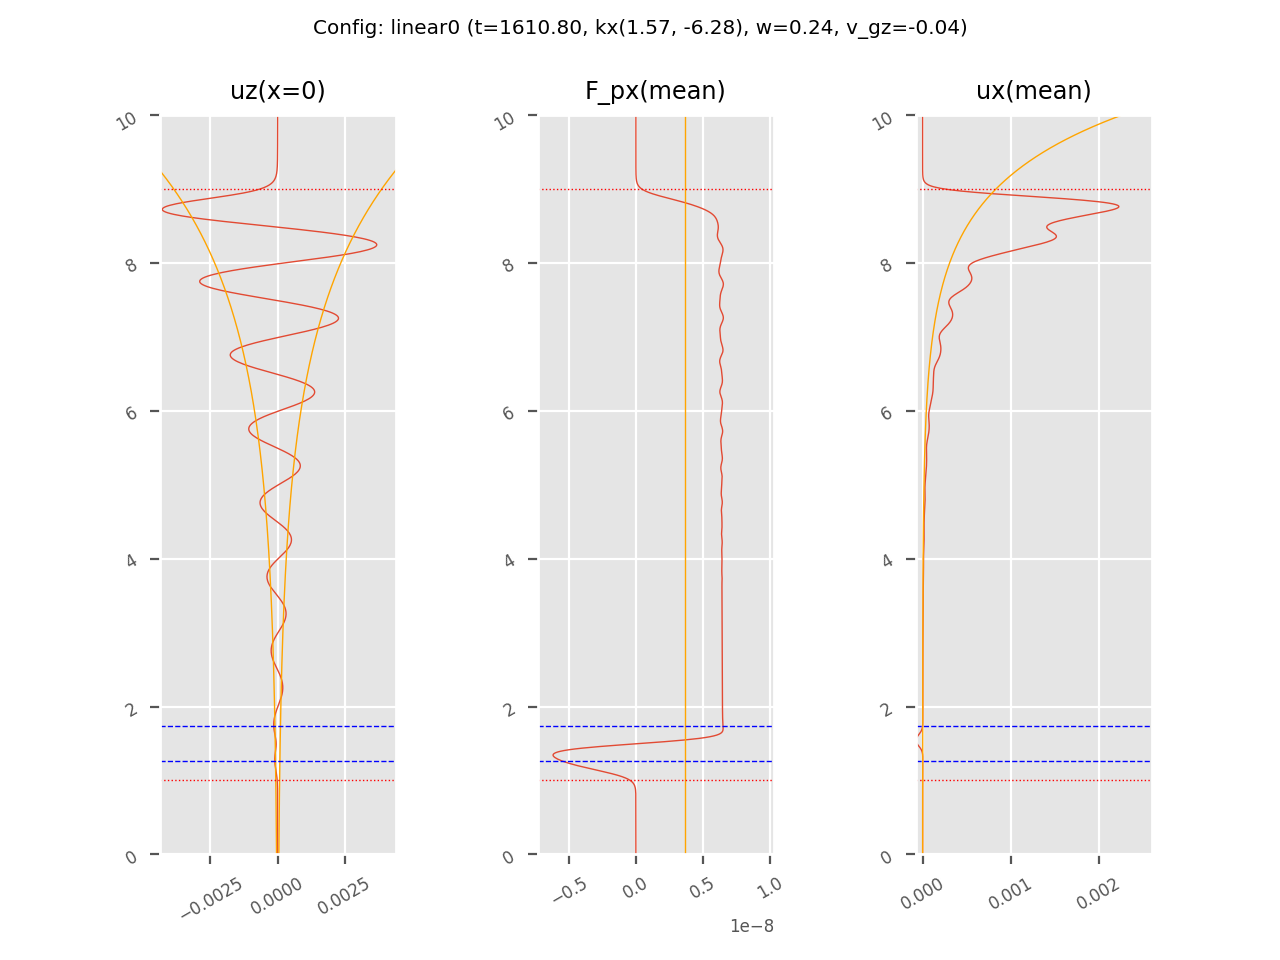
\includegraphics[width=0.5\textwidth]{plots/linear_nonu.png}
    \caption{Snapshot of linear simulation after reaching steady state.
        Analytical predictions of $\abs*{u_z}, \bar{U}_0, S_{px}$ are shown in
        orange. Red dotted lines indicate the onset of the damping region and
        blue dotted lines denote the driving region.}\label{fig:linear_nonu}
\end{figure}
\begin{figure}[t]
    \centering
    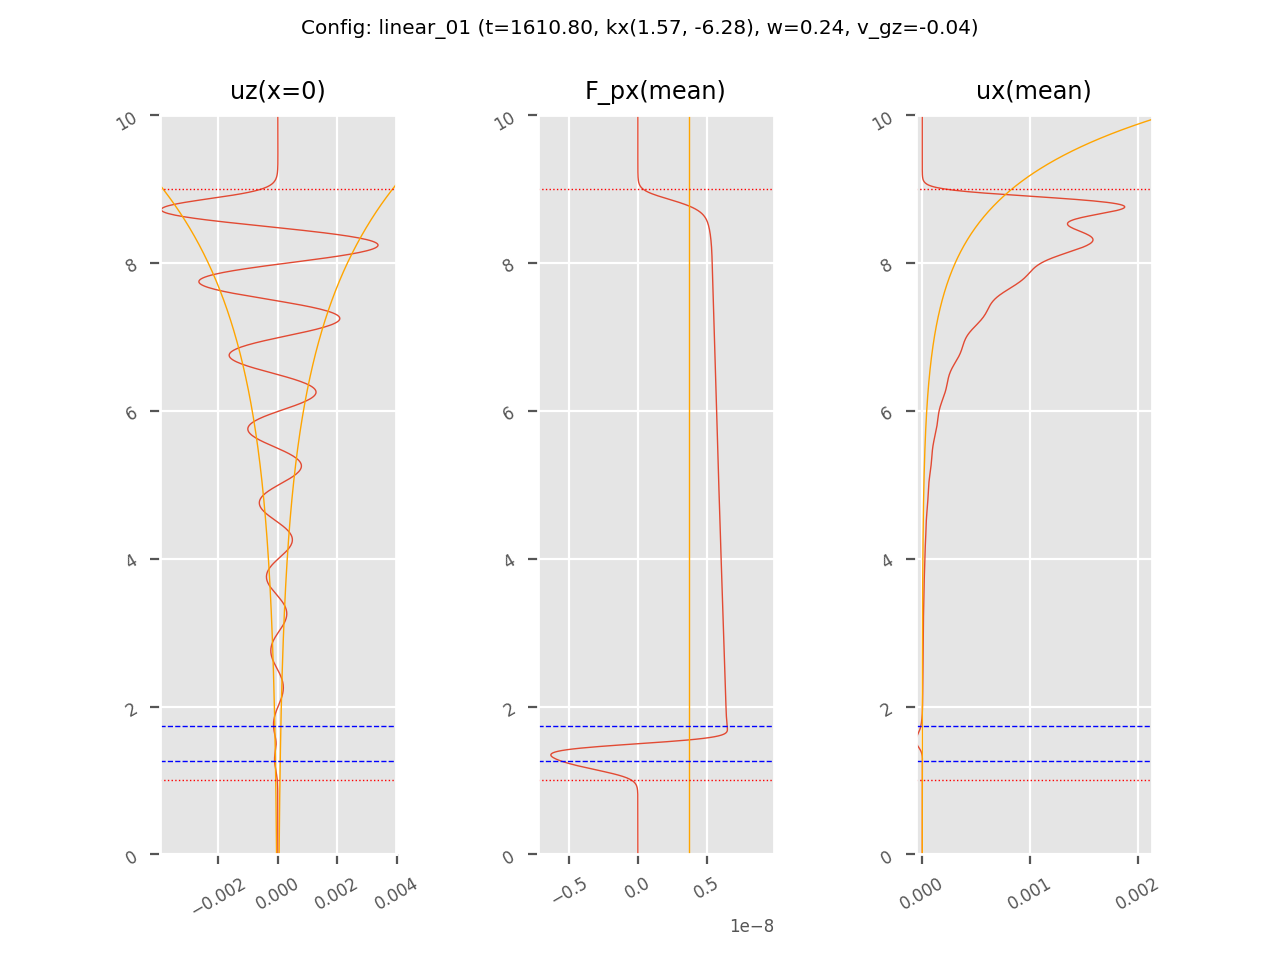
\includegraphics[width=0.5\textwidth]{plots/linear_nu.png}
    \caption{Same as \autoref{fig:linear_nonu} but with $0.3\times $viscosity
    used for nonlinear simulations (YUBONOTE should be the same but that
    simulation mysteriously stopped without me noticing; restarting worked, so
    currently rerunning). Note the slight resulting dissipation in $S_{px}$.
    }\label{fig:linear_nu}
\end{figure}

\subsection{Nonlinear Regime}\label{s:nonlin}

\subsection{Mean Flow Critical Layer Absorption}

In past studies of IGWs in WDs (cite Fuller \& Lai), $\xi_z \equiv
\frac{u_z}{\omega_0}$ the Lagrangian fluid displacement was often used towards
wave breaking criterion $k_{0z}\xi_z \gtrsim 1$. We argue that the wave's
self-interaction via its generated mean flow $\bar{U}_0$ induces total
absorption when the mean flow exceeds critical value
\begin{equation}
    \bar{U}_c = \frac{\omega_0}{k_{0x}}.
\end{equation}
This is consistent with the picture put forth in e.g.\ Goldreich and Nicholson
(cite).

A purely horizontal shear flow $\bar{U}_0(z) \hat{x}$ can be seen in
\autoref{se:fc_orig} to have the effect of modifying time derivatives
$\partial_t$ to their frequency in the comoving frame of the fluid $\partial_t -
\bar{U}_0(z)\partial_x$. For a critical value $\omega_0 - \bar{U}_c k_{0x} = 0$,
the frequency of the linear wave in the fluid's frame of reference vanishes and
critical behavior is observed. In a linear theory or a theory where small scales
are viscosity rather than advection dominated, the incident wave has amplitude
reflection and transmission coefficients
\begin{align}
    \mathcal{R} &= e^{-2\pi \sqrt{\mathrm{Ri} - \frac{1}{4}}}, &
    \mathcal{T} &= e^{-\pi \sqrt{\mathrm{Ri} - \frac{1}{4}}},
    \label{eq:crit_coeffs}
\end{align}
where we have defined Richardson number $\mathrm{Ri} \equiv
\at{\frac{N^2}{\p*{\pd{\bar{U}_0}{z}}^2}}_{z_c}$ at the critical layer $z_c:
\bar{U}_0(z_c) = \frac{\omega_0}{k_{0x}}$. For most shear flows, $\mathrm{Ri}
\gg 1$ and so $\mathcal{R}, \mathcal{T} \ll 1$ and the incident wave is
absorbed.

When the fluid absorbs the incident wave, it absorbs the incident horizontal
momentum flux as well, which is converted into additional horizontal momentum of
the shear flow. Since the shear flow cannot exceed $\bar{U}_c$ the horizontal
phase velocity of the incident wave, the critical layer must thus propagate
downwards (towards the wave source) to accommodate the incident momentum. In
other words, the total horizontal momentum of the shear flow obeys conservation
equation
\begin{equation}
    \pd{}{t}\int\limits_0^{L_z} \rho(z) \bar{U}_0(z, t)\;\mathrm{d}z
        - S_{px} = 0.
\end{equation}
Treating $\bar{U}_0(z > z_c) = \bar{U}_c, \bar{U}(z < z_c) = 0$ gives us exactly
\begin{equation}
    \rho \bar{U}_c\pd{z_c}{t} = -S_{px}.\label{eq:zc_anal}
\end{equation}
For constant $S_{px}$ in space and $\rho \approx \rho_0$, this has analytical
solution
\begin{equation}
    z(t) = -H\ln t - H\ln \frac{H\rho_0(z = 0)c_{ph, x}}{S_{px}}.
\end{equation}

\subsection{Numerical Simulation}

We use the same $k_{0x}, \omega_0$ as \autoref{ss:lin_ns}. Our other parameters
are:
\begin{itemize}
    \item We choose $\nu = 0.35 \frac{\omega_0}{k_{0z}k_{z, \max}}$, where
        $k_{z, \max} = \frac{2\pi N_z}{L_z}$. Note that $\nu =
        \frac{\omega_0}{k_{0z} k_{z, \max}}$ corresponds to the advective term
        $\vec{u} \cdot \vec{\nabla}$ being of the same order as the time
        derivative $\partial_t$ for flow velocities $\vec{u} \sim
        \frac{\omega_0}{k_{0z}}$ at the grid spacing.

    \item We choose $F$ such that $\bar{U}_0(z)$ predicted by
        \autoref{eq:u0_lin} exceeds $\bar{U}_c$ critical velocity for $z <
        L_z$, i.e.\ the wave-induced mean flow is sufficiently large within the
        simulation domain to induce critical layer absorption.
\end{itemize}

Two representative snapshots from our simulation are provided in
\autoref{fig:nl} after the critical layer has had time to form. We may note that
the critical layer, where $S_{px}$ is absorbed and $\bar{U}_0 = \bar{U}_c$,
travels downwards as predicted.
\begin{figure}[t]
    \centering
    \begin{subfigure}{0.5\textwidth}
        \centering
        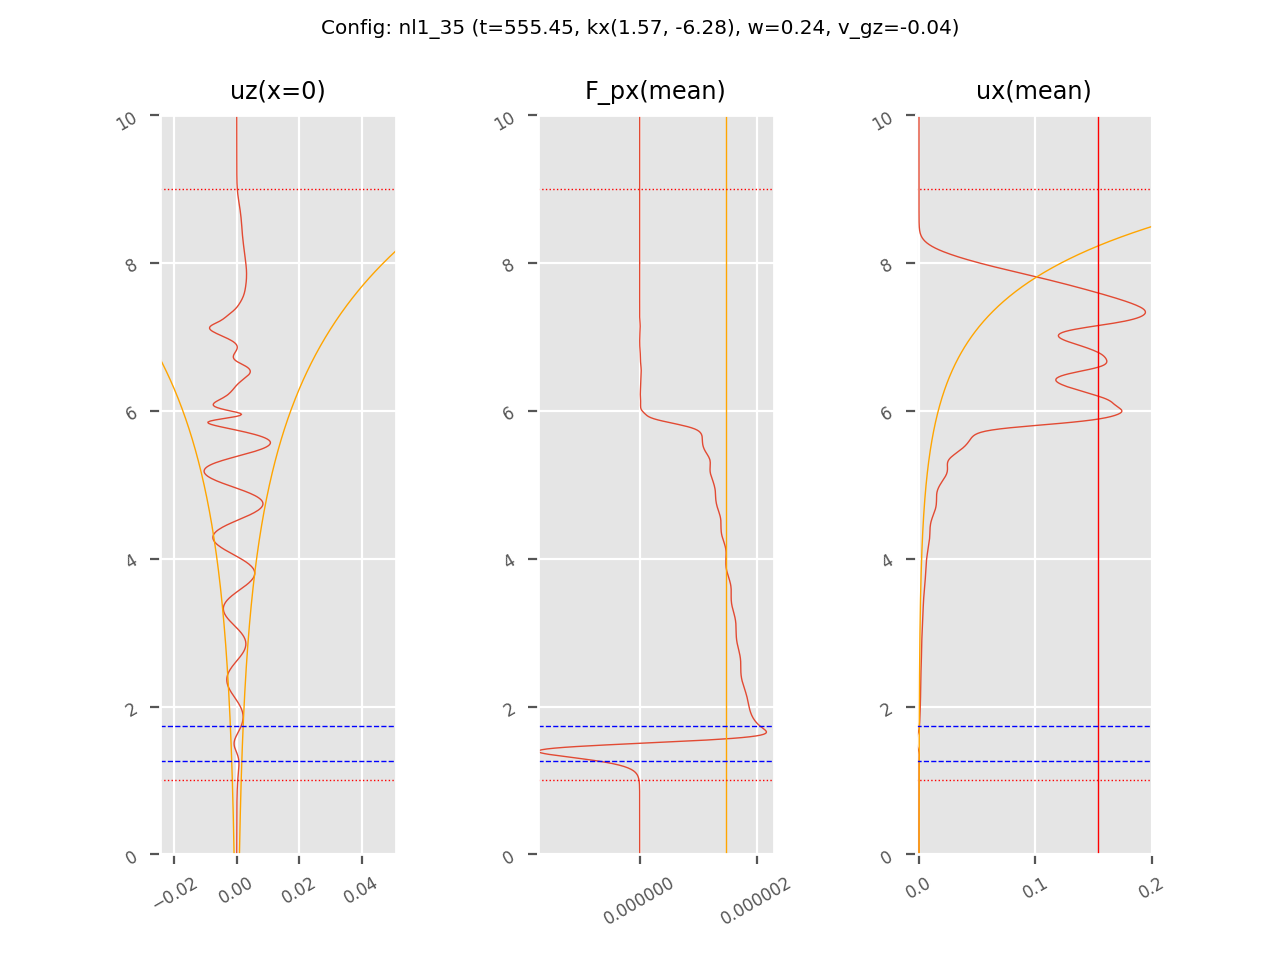
\includegraphics[width=\textwidth]{plots/nl35_1.png}
        \caption{Earlier time snapshot. Legend is the same as
        \autoref{fig:linear_nonu} except $\bar{U}_c$ is marked in red on the
        third panel.}
    \end{subfigure}

    \begin{subfigure}{0.5\textwidth}
        \centering
        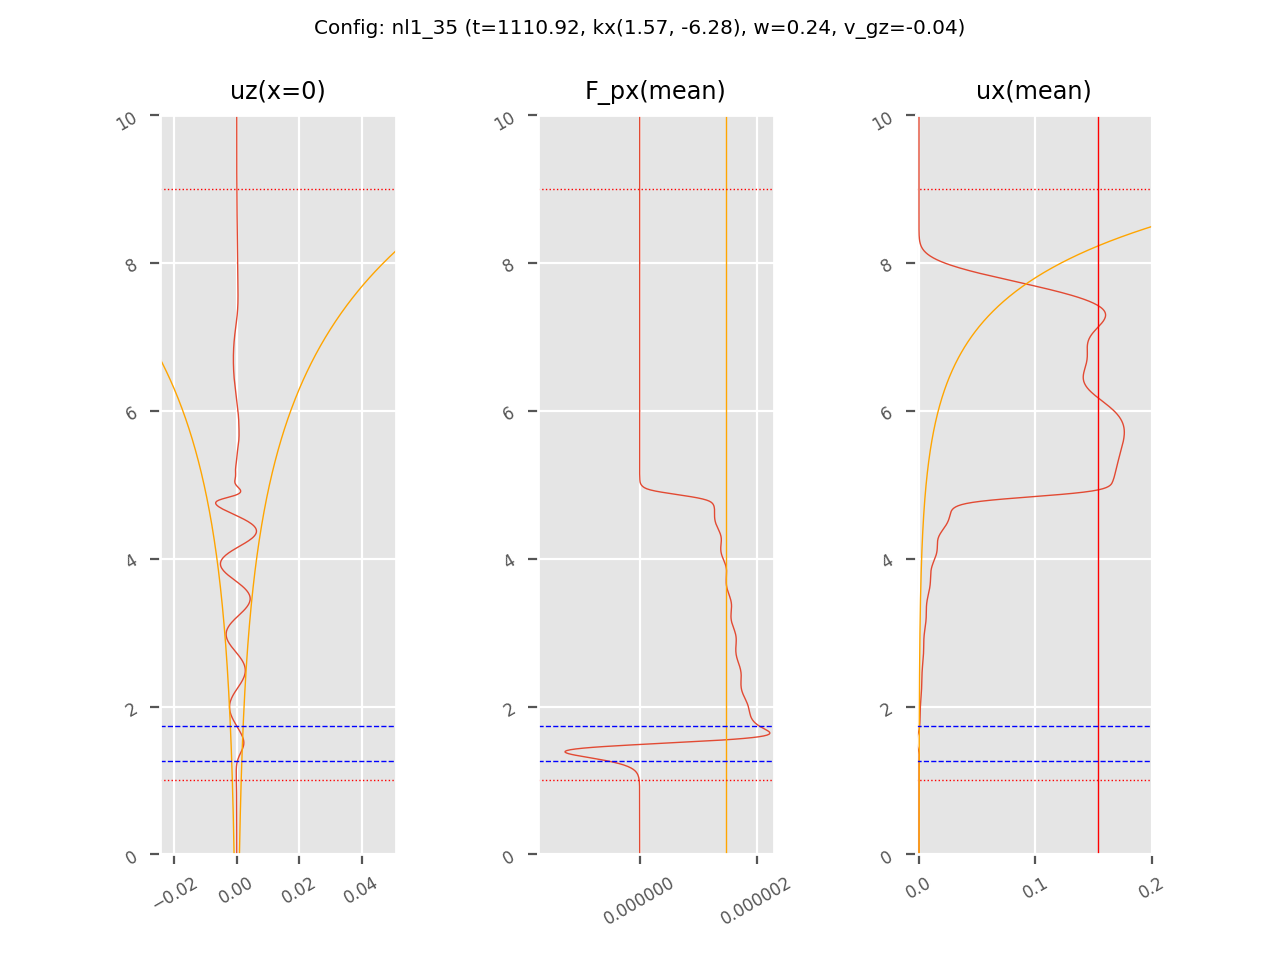
\includegraphics[width=\textwidth]{plots/nl35_2.png}
        \caption{Later snapshot illustrating propagation of $z_c$.}
    \end{subfigure}
    \caption{Nonlinear numerical simulation.}\label{fig:nl}
\end{figure}

\subsection{Propagating Critical Layer}

For the simulation in \autoref{fig:nl}, we may define $z_c = \argmax_z
\pd{\bar{U}_0}{z}$. Computing $\pd{z_c}{t}$ using the analytical flux
\autoref{eq:fpx_lin} allows comparison to \autoref{eq:zc_anal}, which we exhibit
in \autoref{fig:zc_anal}. We see overall good agreement, though some small
deviation is expected since $S_{px}$ is not perfectly conserved owing to
numerical viscosity (and YUBONOTE $S_{px}$ is misestimated?).
\begin{figure}[t]
    \centering
    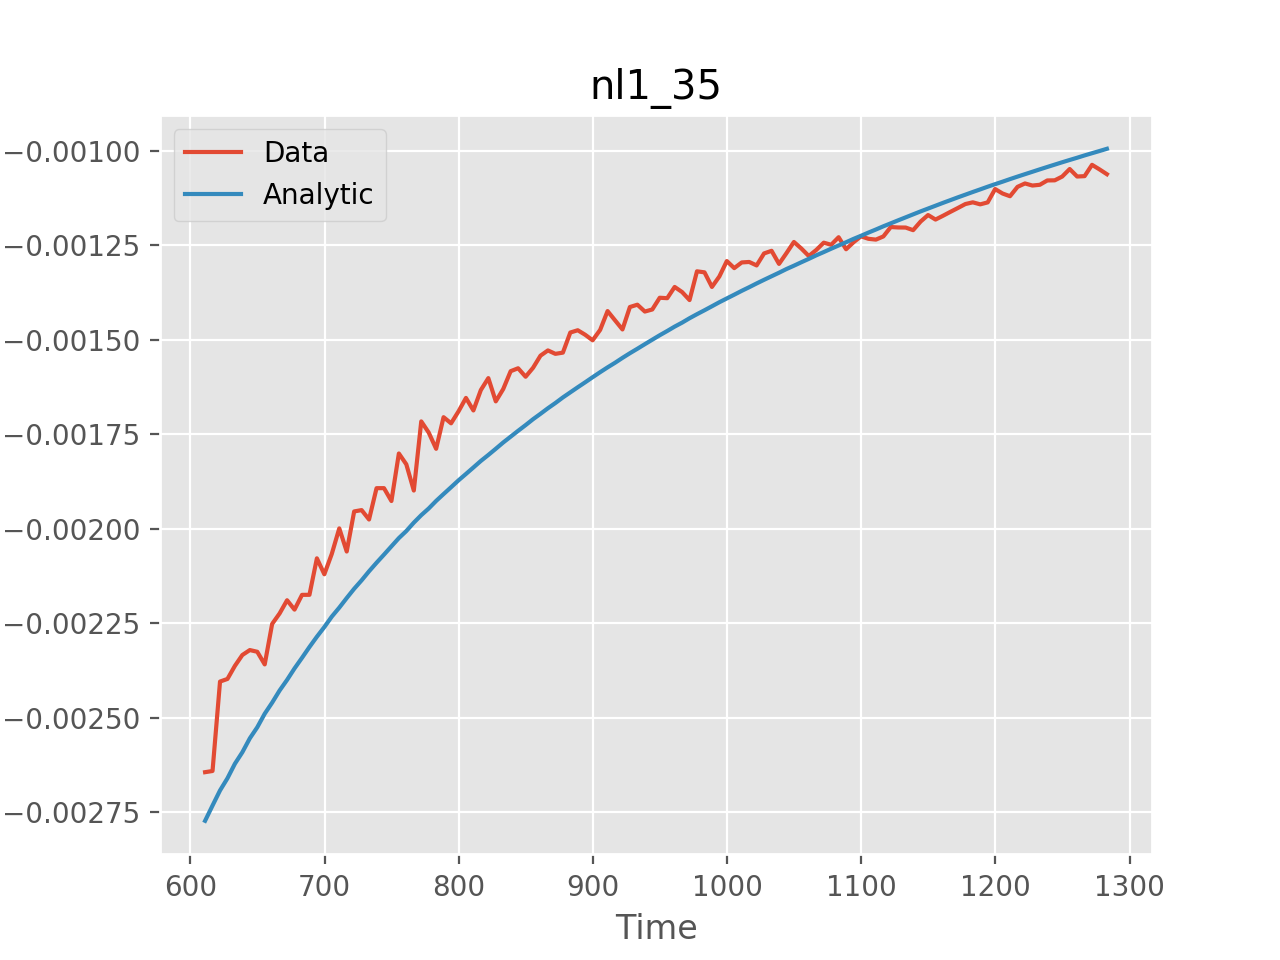
\includegraphics[width=0.5\textwidth]{plots/nl35_front_v.png}
    \caption{Comparison of simulated $\pd{z_c}{t}$ to analytical
    \autoref{eq:zc_anal}. Plot begins after formation of critical layer in
    simulation.}\label{fig:zc_anal}
\end{figure}

However, recalling \autoref{eq:crit_coeffs}, we only expect complete critical
layer absorption when $\mathrm{Ri} \gg \frac{1}{4}$. We may plot $\mathrm{Ri}$
over the same time interval in \autoref{fig:nl35_f_ri}. We may observe that the
Richardson number is initially decreasing but eventually levels out and
begins to increase again. This corresponds to an increasingly sharp critical
layer transition then subsequently a decreasingly sharp critical layer
transition.
\begin{figure}[t]
    \centering
    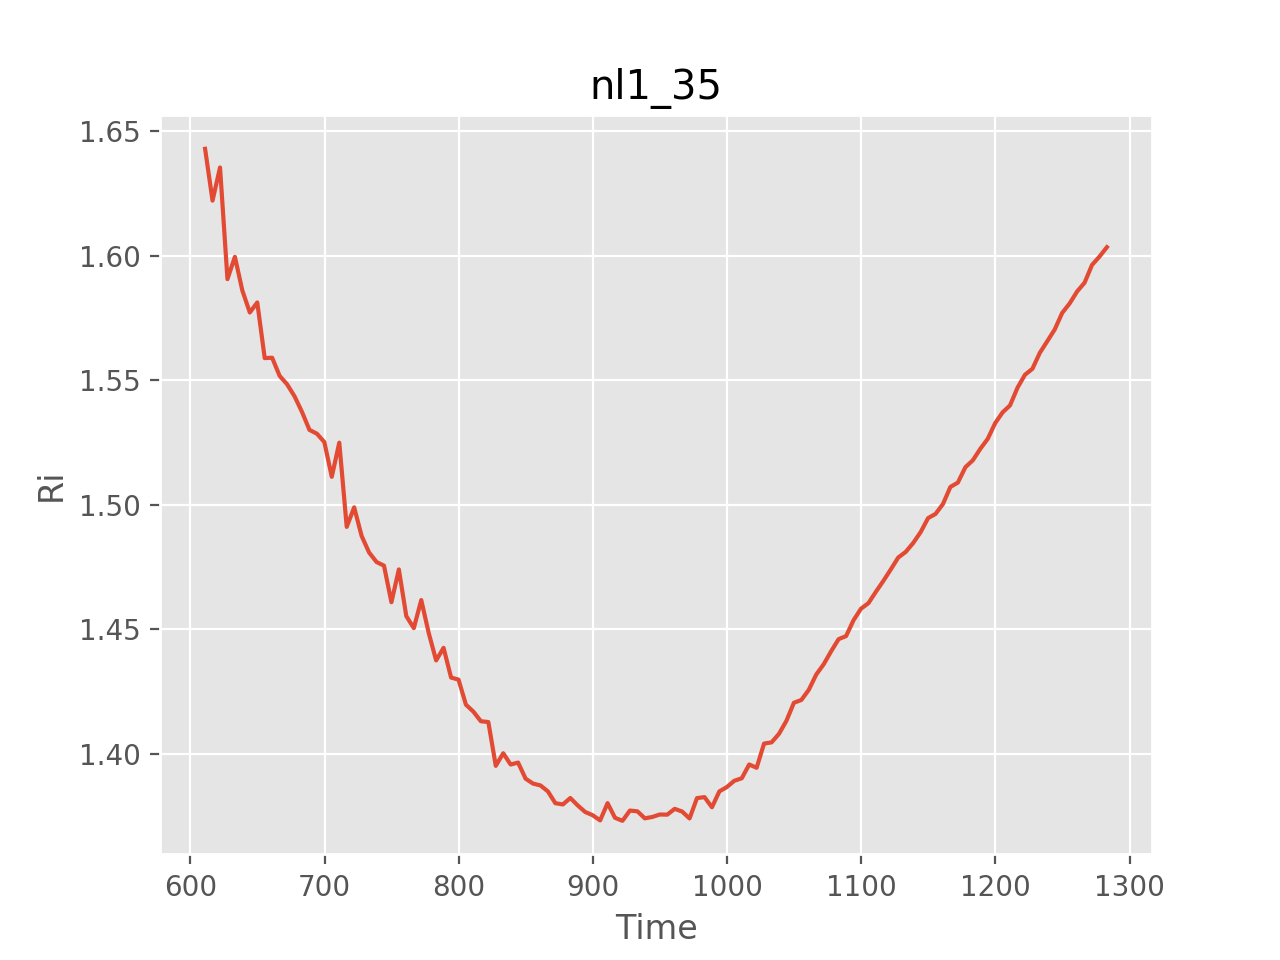
\includegraphics[width=0.5\textwidth]{plots/nl35_f_ri.png}
    \caption{Plot of $\mathrm{Ri}_{\max}(t) = \max_z
    \frac{N^2}{\bar{U}_0'}(t)$ over the simulation time.}\label{fig:nl35_f_ri}
\end{figure}

We argue that the Richardson number is bounded from below by viscosity. A
repeated simulation with a larger viscosity is shown in \autoref{fig:nl1_f_ri},
where the Richardson number does not go nearly as low.
\begin{figure}[t]
    \centering
    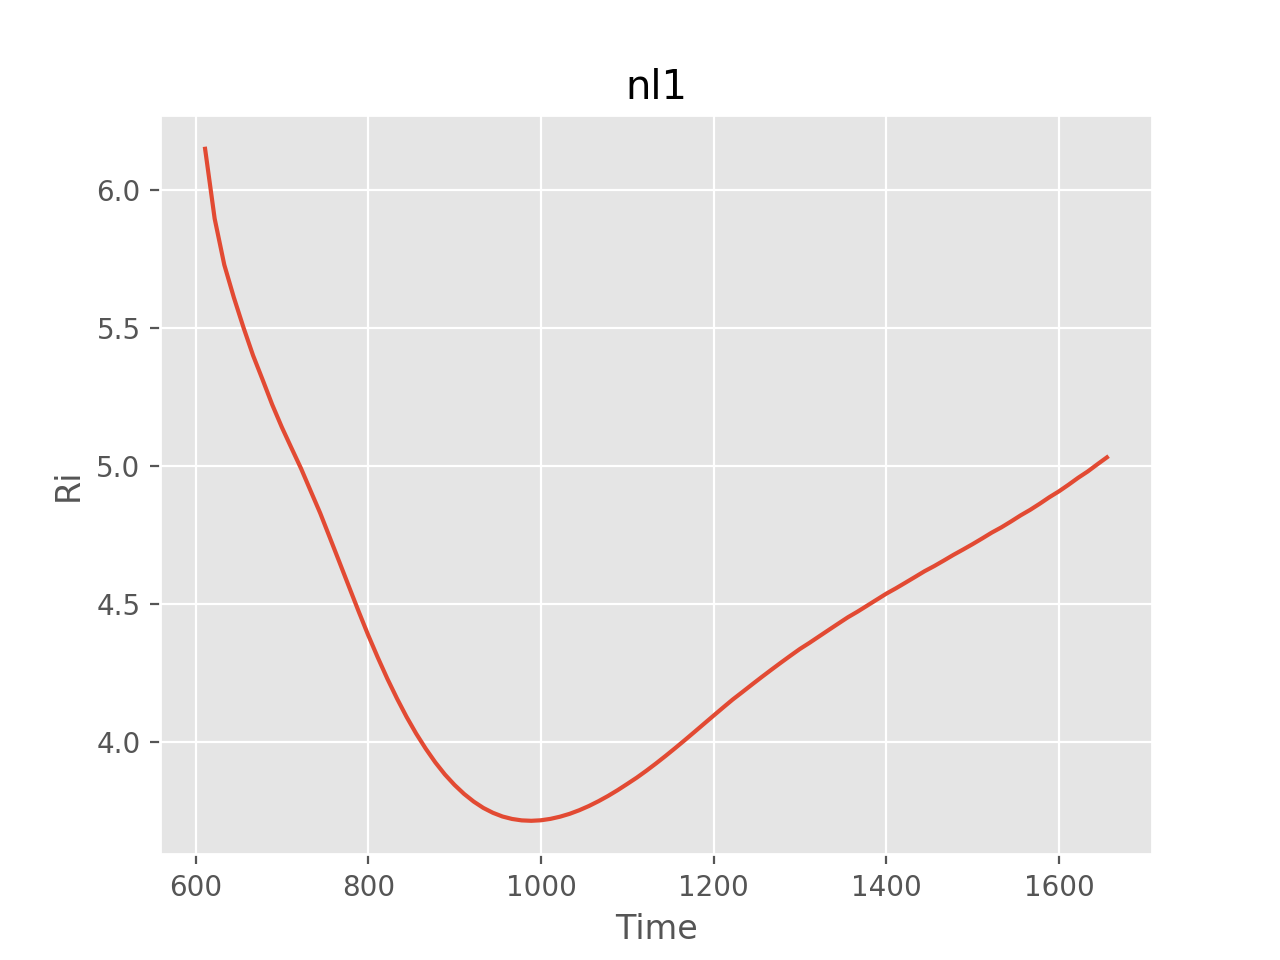
\includegraphics[width=0.5\textwidth]{plots/nl1_f_ri.png}
    \caption{Same as \autoref{fig:nl35_f_ri} but with $\sim 1.3\times$
    viscosity.}\label{fig:nl1_f_ri}
\end{figure}

\clearpage
\onecolumngrid
\appendix

\section{Equation Implementations}\label{ss:strat_impl}

We denote $x \in [0, L_x], z \in [0, L_z]$ the simulation domain and $N_x, N_z$
the number of spectral modes in the respective dimensions. We perform direct
numerical simulation of \autoref{eq:vol_drive} with the open-source
pseudo-spectral code Dedalus (CITE).

Numerically, the nonlinear $\frac{\vec{\nabla}P}{\rho}$ term is problematic: we
desire a system where the fluid fields are not divided by one another. We
introduce $\varpi = \frac{P}{\rho}$ instead, then mandate $\rho_0, \varpi_0$
background fields satisfy hydrostatic equilibrium $\vec{\nabla}\varpi_0 +
\varpi_0 \vec{\nabla}\rho_0 + g\hat{z} = 0$. Taking isothermal stratification,
we find $\varpi_0 = gH$. We further change variables to $\Upsilon = \ln \rho -
\ln \rho_0$ and $\varpi_1 = \varpi - \varpi_0$ deviations from the background
state to obtain a system of equations at most quadratic in fluid fields:
\begin{subequations}\label{se:fc_var}
    \begin{align}
        \vec{\nabla} \cdot \vec{u} &= 0,\\
        \pd{\Upsilon}{t} + \p*{\vec{u} \cdot \vec{\nabla}} \Upsilon
            - \frac{u_z}{H} &= 0,\\
        \pd{u_x}{t} + \p*{\vec{u} \cdot \vec{\nabla}}u_x
            + \pd{\varpi_1}{x} + gH\pd{\Upsilon}{x}
            + \varpi_1 \pd{\Upsilon}{x} &= 0,\\
        \pd{u_z}{t} + \p*{\vec{u} \cdot \vec{\nabla}}u_z
            + \pd{\varpi_1}{z} + gH\pd{\Upsilon}{z}
            + \varpi_1 \pd{\Upsilon}{z} - \frac{\varpi_1}{H} &= 0.
    \end{align}
\end{subequations}
It bears noting that these equations are exactly equivalent to the original
Euler equations and hence conserve horizontal momentum.

\subsection{Artificial Dissipation}

The nonlinear terms in the above equations will transfer energy from lower
wavenumbers to higher wavenumbers. Since spectral codes have no numerical
dissipation, artificial dissipation must be added. To ensure the dissipitive
system conserves horizontal momentum, we begin by adding dissipitive terms to
the flux-conservative form of the Euler fluid equations \autoref{se:fc_orig} (we
use stress tensor $\tau_{ij} = P\delta_{ij}$):
\begin{subequations}
    \begin{align}
        \vec{\nabla} \cdot \vec{u} &= 0,\\
        \partial_t \rho + \vec{\nabla} \cdot (\rho \vec{u} - \nu
            \vec{\nabla}(\rho - \rho_0)) &= 0,\label{eq:visc_cons_mom}\\
        \partial_t (\rho \vec{u}) + \vec{\nabla} \cdot (\rho \vec{u} \vec{u} +
            \mathrm{diag}(\rho \varpi) - \nu \rho \vec{\nabla}\vec{u}) + \rho g
            \hat{z} &= 0.
    \end{align}
\end{subequations}
The same $\nu$ is used for both the diffusive and viscous term, though this is
not required. Since the dissipation is not physical and is purely used for
numerical stability, we choose it such that hydrostatic equilibrium is not
modified. Some algebraic manipulation to re-cast it in the form of
\autoref{se:fc_var} gives
\begin{subequations}
    \begin{align}
        \vec{\nabla} \cdot \vec{u} &= 0,\\
        \partial_t \Upsilon + \p*{\vec{u} \cdot \vec{\nabla}} \Upsilon -
            \frac{u_z}{H} - \nu\p*{\nabla^2 \Upsilon + \p*{\vec{\nabla}
            \Upsilon} \cdot \p*{\vec{\nabla}\Upsilon} - \frac{2}{H}\partial_z
            \Upsilon + \frac{1 - e^{-\Upsilon}}{H^2}} &= 0,\\
        \partial_t \vec{u} + \p*{\vec{u} \cdot \vec{\nabla}}\vec{u} +
            \vec{\nabla} \varpi + \varpi \vec{\nabla} \Upsilon - \nu \nabla^2
            \vec{u} + \vec{u} \nu\p*{\nabla^2 \Upsilon + \p*{\vec{\nabla}
            \Upsilon} \cdot \p*{\vec{\nabla}\Upsilon} - \frac{2}{H}\partial_z
            \Upsilon + \frac{1 - e^{-\Upsilon}}{H^2}}&{}\nonumber\\
        - 2\nu \p*{\p*{\p*{\vec{\nabla}\Upsilon} \cdot \vec{\nabla}}\vec{u} -
            \frac{1}{H}\partial_z \vec{u}} - \frac{\varpi_1}{H} &= 0.
    \end{align}
\end{subequations}
Hydrostatic equilibrium is still $\vec{\nabla} \varpi_0 + g\hat{z} = 0$ where
$\rho = \rho_0, \vec{u} = 0$. Including the damping layers and forcing terms as
described in \autoref{ss:numerics}, we finally obtain the full system of
equations as simulated in Dedalus:
\begin{subequations}
    \begin{align}
        \vec{\nabla} \cdot \vec{u} ={}& 0,\\
        \partial_t \Upsilon - \frac{u_z}{H}
            ={}& \nu\p*{\nabla^2 \Upsilon + \p*{\vec{\nabla}
            \Upsilon} \cdot \p*{\vec{\nabla}\Upsilon} - \frac{2}{H}\partial_z
            \Upsilon + \frac{1 - e^{-\Upsilon}}{H^2}},\nonumber\\
            & - \p*{\vec{u} \cdot \vec{\nabla}}\Upsilon
                -\Gamma(z) \Upsilon
                + \frac{F}{\rho_0(z)}e^{-\frac{(z - z_0)^2}{2\sigma^2}}
                    \cos \p*{k_xx - \omega t},\\
        \pd{u_x}{t} + \pd{T}{x} + gH\pd{\Upsilon}{x} ={}&
            \nu \nabla^2 u_x
            - u_x \nu\p*{\nabla^2 \Upsilon + \p*{\vec{\nabla} \Upsilon} \cdot
                \p*{\vec{\nabla}\Upsilon} - \frac{2}{H}\partial_z \Upsilon
                + \frac{1 - e^{-\Upsilon}}{H^2}}\nonumber\\
            &+ 2\nu \p*{\p*{\p*{\vec{\nabla}\Upsilon} \cdot \vec{\nabla}}u_x
                - \frac{1}{H}\partial_z u_x}
            -\Gamma(z) u_x
                - \p*{\vec{u} \cdot \vec{\nabla}}u_x
                - T_1 \pd{\Upsilon}{x},\\
        \pd{u_z}{t} + \pd{T}{z} + gH\pd{\Upsilon}{z} - \frac{T_1}{H} ={}&
            \nu \nabla^2 u_z
            - u_z \nu\p*{\nabla^2 \Upsilon + \p*{\vec{\nabla} \Upsilon} \cdot
                \p*{\vec{\nabla}\Upsilon} - \frac{2}{H}\partial_z \Upsilon
                + \frac{1 - e^{-\Upsilon}}{H^2}}\nonumber\\
            &+ 2\nu \p*{\p*{\p*{\vec{\nabla}\Upsilon} \cdot \vec{\nabla}}u_z -
                \frac{1}{H}\partial_z u_{z}}
            -\Gamma(z) u_z - \p*{\vec{u} \cdot \vec{\nabla}}u_z
            - T_1 \pd{\Upsilon}{z},\\
        \Gamma(z) &= 7.5\s*{2 + \tanh \frac{z - z_T}{(L_z - z_T) / 2}
            + \tanh \frac{z_B - z}{z_B / 2}},\label{eq:Gamma}
    \end{align}
\end{subequations}

\bibliographystyle{apsrev4-1} % chktex 8
\bibliography{paper}
\end{document}

